\documentclass[11pt]{amsart}
\usepackage[margin=1.15in]{geometry}
\usepackage{amsmath,amssymb,amsthm,tikz,hyperref,booktabs}
\newtheorem{theorem}{Theorem}
\newtheorem{lemma}[theorem]{Lemma}
\newtheorem{proposition}[theorem]{Proposition}
\newtheorem{corollary}[theorem]{Corollary}
\theoremstyle{definition}
\newtheorem{definition}[theorem]{Definition}
\theoremstyle{remark}
\newtheorem*{remark}{Remark}
\newcommand{\abar}{\bar a}
\newcommand{\bbar}{\bar b}
\newcommand{\Irr}{\mathrm{Irr}}

\title{Catalan numbers on the slit plane: combinatorial proofs}
\author{Vamshi Jandhyala}
\date{27 November 2026}

\begin{document}
\begin{abstract}
A walk on the slit plane starts at the origin and never returns to the half-line $\{(-k,0):k\ge0\}$. Square-lattice
walks of length $2n+1$ on the slit plane that end at $(0,1)$ number $4^nC_n$, and several neighbouring endpoints give
similar Catalan formulas. These were found by Bousquet-M\'elou and Schaeffer by solving functional equations, and
Stanley lists them among his bijective proof problems as ones for which a combinatorial proof may not be known. We give
combinatorial proofs of six of the seven formulas so marked, and reduce the seventh, 237(b), to 237(a), whose
combinatorial proof we have not located. The tools are a
classical way of sorting a sequence into cycles, applied to the pieces of a walk between its visits to the
horizontal axis, and a few sign-reversing involutions on pairs of Dyck paths. None of the proofs is a direct
bijection; each is a count of finite sets.
\end{abstract}
\maketitle

\section{The question}

A \emph{square walk} uses the steps $E=(1,0)$, $W=(-1,0)$, $N=(0,1)$ and $S=(0,-1)$. It lives on the \emph{slit plane}
if it starts at the origin and, once it has left, never visits a point $(-k,0)$ with $k\ge0$. Write $a_{i,j}(n)$ for the
number of such walks of length $n$ ending at $(i,j)$, and $\abar_{i,j}(n)$ for the number of walks that instead avoid
only the points $(-k,0)$ with $k>0$ (the origin may be revisited). A \emph{diagonal walk} uses the steps $(\pm1,\pm1)$,
and $b_{i,j}(n)$, $\bbar_{i,j}(n)$ are defined in the same way. Write $C_n=\frac1{n+1}\binom{2n}n$.

Stop and try the smallest case. Of the walks of length $3$ ending at $(0,1)$, exactly four stay on the slit plane:
\[
  ENW,\qquad NEW,\qquad NWE,\qquad NNS .
\]
(A walk such as $WNE$ fails at once, and $NSN$ returns to the origin.) Four is $4^1C_1$. Stanley's list of bijective
proof problems \cite[Problems 236, 237]{Bij} collects the following counts, found by Bousquet-M\'elou and Schaeffer
\cite{BMS}, Bousquet-M\'elou \cite{BM} and Xin \cite{Xin}, all with generating functions:
\begin{align*}
  &\text{236(a) } a_{0,1}(2n+1)=4^nC_n, &&\text{(b) } a_{1,0}(2n+1)=C_{2n+1}, &&\text{(c) } a_{-1,1}(2n)=\tfrac12C_{2n},\\
  &\text{(d) } a_{1,1}(2n)=4^{n-1}C_n+\tfrac12C_{2n}, &&\text{(e) } \abar_{0,0}(2n)=2\cdot4^nC_n-C_{2n+1};\\
  &\text{237(a) } b_{1,1}(2n+1)=C_{2n+1}, &&\text{(b) } b_{-1,1}(2n+1)=2\cdot4^nC_n-C_{2n+1}, &&\text{(c) } b_{0,2}(2n)=C_{2n}\ (n\ge1),\\
  &\text{(d) } b_{2i,0}(2n)=\tfrac in\tbinom{2i}i\tbinom{2n}{n-i}4^{n-i}\ (1\le i\le n), &&\text{(e) } \bbar_{0,0}(2n)=4^nC_n.
\end{align*}
Here (c) and (d) of 236 hold for $n\ge1$, while $b_{0,2}(0)=0$, and $b_{2i,0}(2n)=0$ for $i>n$. Stanley marks 236(a), (c), (d), (e) and 237(b), (d), (e) with $[?]$:
``uncertain whether a combinatorial proof is known''. Item 236(b) has a bijective proof by Barcucci, Pergola, Pinzani
and Rinaldi \cite{BPPR}, and 237(d) with $i=1$ follows from the cycle lemma \cite[Prop.~7]{BM}; Nadeau gave a general bijection for the
smallest endpoint on the positive axis, which covers both \cite{Nad}. Items 237(a) and (c)
carry no $[?]$ in the list; we have not located their combinatorial proofs, and Bousquet-M\'elou and Schaeffer asked
for a combinatorial explanation of the diagonal count $C_{2n+1}$ \cite[remark after Thm.~8]{BMS}. Bousquet-M\'elou wrote
that ``Algebraic generating functions and Catalan numbers call for `classical' (if not bijective) combinatorial
proofs'' \cite[Sect.~1]{BM}, and that the cycle lemma ``usually only works for walks ending at a specific
position''.

\begin{theorem}\label{thm:main}
There are combinatorial proofs, by finite bijections, sign-reversing involutions and double counting, of 236(a), (b),
(c), (d), (e) and 237(d), (e), and of the identity
\[
  b_{1,1}(2n+1)+b_{-1,1}(2n+1)=2\cdot4^nC_n .
\]
Together with any combinatorial proof of 237(a), the identity gives 237(b).
\end{theorem}

The formulas are not new, and neither are several of the steps: Corollary~\ref{cor:T} is Bousquet-M\'elou's
cycle-lemma proof of 236(b) \cite[Prop.~2]{BM}, cycle sorting is classical, and the odd-cycle recolouring in
Proposition~\ref{prop:loops} adapts Spivey's involution \cite{Sp}, with the parity of a cycle's total semilength in
place of its length. What is new is the identification of barred loops with signed pairs of Dyck paths
(Proposition~\ref{prop:loops}), which gives 236(a), (c), (e), and the cycle-sorting proofs of 236(d), of 237(e), of
237(d) with $i\ge2$ and of the identity behind 237(b); the case $i=1$ of 237(d) was already covered \cite{BM,Nad}.
The proofs are not bijections from walks to Catalan objects. The main tool
counts walks by cutting them at their visits to the horizontal axis and sorting the pieces into cycles, with weight $1/k$
for a cycle of $k$ pieces. This is a combinatorial form of the factorisation that Bousquet-M\'elou uses with logarithms
of generating functions \cite[Props.~8, 9]{BM}, and of an old idea of Spitzer \cite{St}; we say more about the relation
in Section~\ref{sec:remarks}. The new ingredient is the identification, by a sign-reversing involution, of the loops
on the barred slit plane with signed pairs of Dyck paths (Proposition~\ref{prop:loops}). From it, $a_{0,1}(2n+1)$ turns
out to be the even-index Catalan convolution $\sum_kC_{2k}C_{2n-2k}$, which equals $4^nC_n$ by Shapiro's identity, and
Hajnal and Nagy \cite{HN} gave that identity a bijective proof.

Two conventions run through the note. A Dyck path of semilength $r$ is \emph{irreducible} if it returns to height zero
only at its end; irreducible Dyck paths of semilength $r\ge1$ number $C_{r-1}$. And all sums are finite: no step uses a
power series.

\section{Pieces, cycles and cyclic weights}\label{sec:cycles}

\begin{definition}
A class of \emph{atoms} is a set of objects, each with a positive integer \emph{size}, an integer \emph{increment} and
a sign $\pm1$, with finitely many atoms of each size. A \emph{word} is a finite sequence of atoms; its size, increment
and sign are the sum, sum and product over its atoms. Its \emph{partial increments} are the increments of its nonempty
prefixes. The \emph{cyclic weight} of the class is
\begin{equation}\label{eq:cw}
  c(m,d)=\sum_{w}\frac{\operatorname{sign}(w)}{k(w)},
\end{equation}
the sum over nonempty words $w$ of size $m$ and increment $d$, where $k(w)$ is the number of atoms of $w$.
\end{definition}

The weight $1/k$ counts cycles. Rotating a word of $k$ atoms gives $k$ words (with repetitions if the word is periodic),
so $c(m,d)$ is the number of cyclic arrangements of atoms, each counted with weight one over its period's number of
symmetries. Labels make this precise and remove the fractions, as follows.

Fix a word of $K$ atoms and attach to its atoms $K$ distinct labels from $\{1,\dots,K\}$. A \emph{labelled cycle} is a
cyclic sequence of distinctly labelled atoms; it has exactly $k$ rotations, all different, because the labels differ.

\begin{lemma}[Cycle sorting]\label{lem:sort}
Let $K\ge0$ and fix a class of atoms.
\begin{enumerate}
\item[(i)] Labelled words of $K$ atoms whose partial increments are all $\ge0$ and whose increment is $0$ are in bijection
with sets of labelled cycles, using each label once, in which every cycle has increment $0$.
\item[(ii)] Labelled words of $K$ atoms whose partial increments are all $>0$ are in bijection with sets of labelled
cycles, using each label once, in which every cycle has positive increment.
\end{enumerate}
Both bijections preserve the multiset of atoms.
\end{lemma}

\begin{proof}
(i) Given a set of cycles of increment $0$, read each cycle from a position where its running increment is minimal,
choosing among such positions the one whose next atom has the least label; call that label the \emph{root}. Each cycle,
so read, is a word with partial increments $\ge0$ and increment $0$. Concatenate the cycles in decreasing order of
root. The result has partial increments $\ge0$ and increment $0$.

To invert, scan the word and look at the atoms that start at height $0$ (the first atom, and every atom following a
prefix of increment $0$). Cut the word in front of each such atom whose label is smaller than every label seen so far at
height $0$. The root of a cycle is the least label among its own height-$0$ atoms, and the roots decrease from one cycle
to the next, so these record minima are exactly the roots; cutting at them recovers the cycles, and reading each piece
cyclically recovers the cycles themselves.

(ii) Let a cycle have $k$ atoms and increment $d>0$, and put $p=d/k$. Subtract $p$ from the increment of every atom.
The adjusted cycle has increment $0$; read it from a position of minimal adjusted running increment, breaking ties by
the least next label, as in (i). Every prefix of $\ell$ atoms of this reading then has actual increment at least
$p\ell>0$. Concatenate the cycles in increasing order of slope $p$, and among cycles with equal slope in decreasing order
of root. The partial increments of the result are positive.

To invert, draw the partial increments of the word as points $(\ell,s_\ell)$, $0\le\ell\le K$, and take the greatest
convex function below them. Its faces have the slopes $p$ of the cycles in increasing order: a cycle read from a minimum
of its adjusted increments lies on or above the line of slope $p$ through its start and returns to it at its end, and
slopes increase from cycle to cycle. On each face, cut at the record-minimum labels among the atoms that start on the
face, exactly as in (i). A word with positive partial increments has a positive first slope, so every recovered cycle
has positive increment.
\end{proof}

This is the combinatorial lemma of Spitzer and Bohnenblust, in the form surveyed by Steele \cite{St}; part (ii) is the
convex-minorant version, with ties between equal slopes handled as by Abramson and Pitman \cite{AP}. The consequence we
use is a counting formula.

\begin{lemma}\label{lem:count}
For a class of atoms with cyclic weight $c$, the signed number of words of size $N$ whose partial increments are $\ge0$
and whose increment is $0$ is
\[
  \sum_{q\ge0}\frac1{q!}\sum_{\substack{m_1+\dots+m_q=N\\ m_j\ge1}}\ \prod_{j=1}^q c(m_j,0),
\]
where the term $q=0$ is $1$ if $N=0$ and $0$ otherwise. The signed number of words of size $N$ and increment $D>0$
whose partial increments are positive is the same sum with $c(m_j,0)$ replaced by $c(m_j,d_j)$ and an extra sum over
$d_1+\dots+d_q=D$ with all $d_j\ge1$.
\end{lemma}

\begin{proof}
Count labelled words of $K$ atoms both ways in Lemma~\ref{lem:sort}. On the cycle side, order the $q$ cycles, with
$k_1,\dots,k_q$ atoms. Distributing the $K$ labels over the cyclic positions gives $K!/(k_1\cdots k_q)$ labelled
configurations for each choice of the underlying unlabelled words read from a fixed start: dividing by $k_j$ forgets
where cycle $j$ starts. Divide by $q!$ to forget the order of the cycles and by $K!$ to forget the labels, then sum over
$K$ and the $k_j$. Every sum is finite.
\end{proof}

So two classes of atoms with equal cyclic weights have equally many words of each size under either constraint. That is
how walks will be compared with paths below. Figure~\ref{fig:loop} shows the pieces of a walk.

\begin{figure}[ht]
\centering
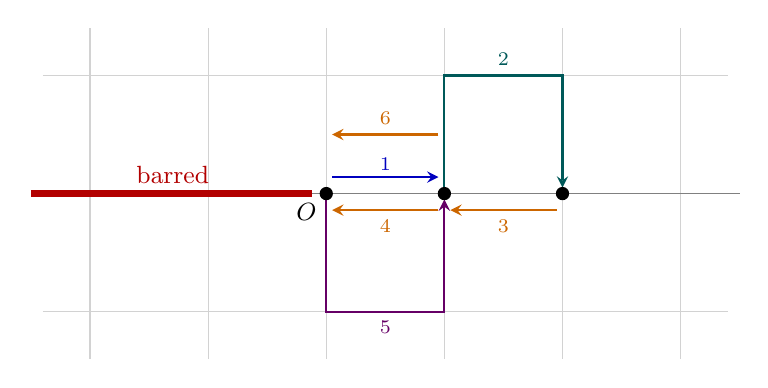
\begin{tikzpicture}[scale=1.5,>=stealth]
  \draw[gray!35] (-2.4,-1.4) grid (3.4,1.4);
  \draw[gray] (-2.5,0)--(3.5,0);
  \draw[line width=2.4pt,red!70!black] (-2.5,0)--(-0.12,0);
  \node[red!70!black,above] at (-1.3,0) {\small barred};
  \draw[thick,->,blue!75!black] (0.05,0.14)--(0.95,0.14);
  \node[blue!75!black,font=\scriptsize] at (0.5,0.25) {1};
  \draw[thick,->,teal!70!black] (1,0.05)--(1,1)--(2,1)--(2,0.05);
  \node[teal!70!black,font=\scriptsize,above] at (1.5,1) {2};
  \draw[thick,->,orange!80!black] (1.95,-0.14)--(1.05,-0.14);
  \node[orange!80!black,font=\scriptsize,below] at (1.5,-0.14) {3};
  \draw[thick,->,orange!80!black] (0.95,-0.14)--(0.05,-0.14);
  \node[orange!80!black,font=\scriptsize,below] at (0.5,-0.14) {4};
  \draw[thick,->,violet!80!black] (0,-0.05)--(0,-1)--(1,-1)--(1,-0.05);
  \node[violet!80!black,font=\scriptsize,below] at (0.5,-1) {5};
  \draw[thick,->,orange!80!black] (0.95,0.5)--(0.05,0.5);
  \node[orange!80!black,font=\scriptsize,above] at (0.5,0.5) {6};
  \foreach \x in {0,1,2} \fill (\x,0) circle (1.6pt);
  \node[below left] at (0,0) {\small $O$};
\end{tikzpicture}
\caption{The loop $E\,NES\,W\,W\,SEN\,W$ on the barred slit plane, cut at its visits to the axis into six atoms,
numbered in order, with increments $+1,+1,-1,-1,+1,-1$. Its partial increments $1,2,1,0,1,0$ are the abscissae of its axis visits; they stay
$\ge0$ because the walk never visits $(-k,0)$ with $k>0$.}
\label{fig:loop}
\end{figure}

\section{Three cyclic weights}\label{sec:weights}

\subsection*{Paths on a line} Let $g_r$ be the cyclic weight of irreducible Dyck paths at semilength $r$ (atoms: the
irreducible Dyck paths, size the semilength, increment $0$), and $h_r$ that of the \emph{primitive bridges}: walks of
length $2r$ with steps $\pm1$ that return to $0$ only at the end, size the semilength. A word of primitive bridges is
a bridge, so
\[
  g_r=\sum_{P}\frac1{k(P)},\qquad h_r=\sum_{B}\frac1{k(B)},
\]
over Dyck paths $P$, respectively bridges $B$, of semilength $r$, where $k$ counts returns to zero.

\begin{lemma}\label{lem:gh}
For $r\ge1$, $\ 2r\,g_r=\binom{2r}r$ and $2r\,h_r=4^r$.
\end{lemma}

\begin{proof}
Dyck paths of semilength $r$ with $k$ returns number $\frac{k}{2r-k}\binom{2r-k}{r}$: removing the first and last step
of each irreducible piece leaves a forest of $k$ ordered full binary trees with $r-k$ internal vertices, and such
forests with $e$ internal vertices number
\begin{equation}\label{eq:forest}
  F(k,e)=\frac{k}{2e+k}\binom{2e+k}{e}
\end{equation}
by the cycle lemma (record $+1$ for an internal vertex and $-1$ for a leaf in preorder; exactly $k$ of the $2e+k$
rotations of such a word are forest codes, periodic words included, by counting marked positions). A bridge with $k$
returns is a Dyck path with $k$ returns in which each irreducible piece is optionally reflected, so
\[
  2r\,g_r=\sum_{k=1}^r\frac{2r}{2r-k}\binom{2r-k}r,\qquad 2r\,h_r=\sum_{k=1}^r2^k\frac{2r}{2r-k}\binom{2r-k}r,
\]
and $\frac{2r}{2r-k}\binom{2r-k}{r}=2\binom{2r-k-1}{r-1}$. Now read a word of length $2r$ in two letters until one
letter has occurred $r$ times, which happens at a unique time $2r-k$ with $1\le k\le r$. There are $2$ choices for that
letter and $\binom{2r-k-1}{r-1}$ for the positions of its earlier occurrences. If the word is arbitrary, its last $k$
letters are free, and the words number $\sum_k2^{k+1}\binom{2r-k-1}{r-1}=4^r$; if it has $r$ of each letter, its last
$k$ letters are forced, and the words number $\sum_k2\binom{2r-k-1}{r-1}=\binom{2r}r$.
\end{proof}

\subsection*{Square walks} A \emph{bilateral atom} is a square walk that starts and ends on the $x$-axis and does not
meet it in between: a single step $E$ or $W$, or an arch above or below the axis. Its size is its length and its
increment its horizontal displacement. A word of bilateral atoms is a walk that ends on the axis; the walk lies on the
slit plane, or on the barred slit plane, exactly when its partial increments are $>0$, respectively $\ge0$
(Figure~\ref{fig:loop}). Let $c_s(m,i)$ be the cyclic weight of bilateral atoms.

\begin{lemma}\label{lem:cs}
For $m\ge1$, $c_s(m,i)=\frac1m\binom{2m}{m-i}$ if $m-i$ is even and $|i|\le m$, and $c_s(m,i)=0$ otherwise.
\end{lemma}

\begin{proof}
Fix $2v$ vertical and $h$ horizontal steps, $m=2v+h$, and first let $v\ge1$. In a cycle of atoms, mark one vertical
step. A cycle with $k$ atoms whose rotation group has order $s$ has weight $1/s$ when counted as an unlabelled
cycle, and exactly $2v/s$ distinct marked versions, because no nontrivial rotation fixes a marked step. So marked
cycles number $2v$ times the cyclic weight. Delete the horizontal steps: what remains is a cycle of primitive bridges in
the vertical direction with one marked step, and by the same count with Lemma~\ref{lem:gh} there are $2v\,h_v=4^v$ of
these. Conversely, the marked step fixes an origin, and the $h$ horizontal steps can be put back into the $2v$ gaps
following the vertical steps in $\binom{m-1}{h}$ ways, with $\binom{h}{(h+i)/2}$ choices of which are $E$; a horizontal
step put back at height $0$ becomes an atom of its own. So the contribution of $v$ is
\[
  \frac{4^v}{2v}\binom{m-1}{h}\binom{h}{(h+i)/2}=\frac1m\binom m{2v}4^v\binom{m-2v}{(m-2v+i)/2},
\]
and for $v=0$ the cycle is $m$ horizontal atoms and the same formula holds. Finally, split a word of length $2m$ in
$\pm$ into $m$ consecutive pairs. The pairs $++$ and $--$ are $E$ and $W$, and a mixed pair has two forms; a word with
$m+i$ plus signs and $2v$ mixed pairs arises once from each term, so the contributions sum to $\frac1m\binom{2m}{m+i}$.
\end{proof}

\section{Loops and signed pairs of Dyck paths}\label{sec:loops}

Let $L_m=\abar_{0,0}(m)$ be the number of loops of length $m$ on the barred slit plane, with $L_0=1$, and $T_m=a_{1,0}(m)$.

\begin{corollary}\label{cor:T}
$T_m=C_m$ for odd $m$ and $T_m=0$ for even $m$; that is, 236(b) holds.
\end{corollary}

\begin{proof}
A word of bilateral atoms with increment $1$ has exactly one rotation, up to equality of words, with positive partial
increments: start after the last position where the running increment is minimal, and no second start works, since the
increments between two good starts would be two positive integers adding to $1$. Such a word is not periodic. So $T_m$
is the number of unlabelled cycles of increment $1$, which is $c_s(m,1)=\frac1m\binom{2m}{m-1}=C_m$ for odd $m$.
This is Bousquet-M\'elou's argument \cite[Prop.~2]{BM}.
\end{proof}

\begin{proposition}\label{prop:loops}
$L_m=\sum_{j=0}^m(-1)^jC_jC_{m-j}$. That is, barred loops of length $m$ are equinumerous with the signed set of
ordered pairs $(A,B)$ of Dyck paths of total semilength $m$, with sign $(-1)^{|B|}$.
\end{proposition}

\begin{proof}
By Lemma~\ref{lem:count}(i), $L_m$ is determined by the cyclic weights $c_s(r,0)$, which by Lemma~\ref{lem:cs} are
$0$ for odd $r$ and $\frac1r\binom{2r}r=2g_r$ for even $r$. Now take the pairs $(A,B)$, cut both paths into irreducible
pieces, colour each piece by the path it came from, and sort all pieces into cycles by Lemma~\ref{lem:sort}(i) (every
piece has increment $0$, and the two paths are recovered by sorting each colour separately). A cycle of total semilength
$r$ in one colour carries sign $+1$ or $(-1)^r$, so cycles have total weight $g_r(1+(-1)^r)$. Cancel the cycles of odd
size: among all cycles of odd size, take the one containing the least label and switch its colour (an adaptation of Spivey's involution for the alternating
convolution of central binomial coefficients \cite{Sp}, with the parity of the total semilength of a cycle in place of
its length). This changes the sign
and keeps the set of odd cycles, so it is a sign-reversing involution, and its fixed points use only even cycles, each in
two colours of sign $+1$. Their cyclic weight is $2g_r$ for even $r$ and $0$ for odd $r$, the same as for loops, and
Lemma~\ref{lem:count} gives equal counts.
\end{proof}

For example $L_2=3$: the loops $EW$, $NS$, $SN$, against the pairs of semilengths $(2,0)$, $(1,1)$, $(0,2)$ counted
$2-1+2$. Split the alternating sum by parity:
\[
  H_n=\sum_{k=0}^nC_{2k}C_{2n-2k},\qquad K_n=\sum_{k=0}^{n-1}C_{2k+1}C_{2n-2k-1}.
\]
Then $L_{2n}=H_n-K_n$, and cutting a Dyck path of semilength $2n+1$ at its first return gives $C_{2n+1}=H_n+K_n$.

\section{Primitive loops and the endpoint $(0,1)$}\label{sec:01}

A barred loop is \emph{primitive} if it is nonempty and returns to the origin only at its end; let $P_m$ count them.
Every barred loop is a sequence of primitive loops.

\begin{lemma}\label{lem:prim}
$P_{2r}=2C_{2r-1}+L_{2r-2}$ for $r\ge1$, and $P_m=0$ for odd $m$.
\end{lemma}

\begin{proof}
All the following are finite signed sets graded by size, and ``$X\cdot Y$'' denotes the signed set of pairs, graded by
total size. Let $\mathcal D$ be Dyck paths (size: semilength, sign $+$), $\mathcal D'$ the same with sign $(-1)^{\rm size}$,
$\mathcal J$ the set consisting of the empty object (sign $+$) and the irreducible Dyck paths (sign $-$), and $\mathcal J'$
the same with an extra sign $(-1)^{\rm size}$. Let $\mathcal L$ be barred loops (size: the length, so that Proposition~\ref{prop:loops} matches grades) and $\mathcal Q$
the empty object (sign $+$) with the primitive loops (sign $-$).

In $\mathcal D\cdot\mathcal J$, if the irreducible part is present, append it to the path; otherwise, if the path is
nonempty, detach its last irreducible piece. This is a sign-reversing involution whose only fixed point is the empty pair,
and the same move works in $\mathcal D'\cdot\mathcal J'$, because it does not change the total size. Likewise
$\mathcal L\cdot\mathcal Q$ cancels to the empty pair by appending or detaching a last primitive loop. Write $|X|_m$ for
the signed size of $X$ in grade $m$. By Proposition~\ref{prop:loops}, $|\mathcal L|_m=|\mathcal D\cdot\mathcal D'|_m$, so
in each grade the signed size of $\mathcal L\cdot\mathcal J\cdot\mathcal J'$ equals that of
$\mathcal D\cdot\mathcal J\cdot\mathcal D'\cdot\mathcal J'$, which is $1$ in grade $0$ and $0$ otherwise. Now count
$\mathcal Q\cdot\mathcal L\cdot(\mathcal J\cdot\mathcal J')$ in grade $m$ in two ways: cancelling the first two factors
leaves $|\mathcal J\cdot\mathcal J'|_m$, and cancelling the last two leaves $|\mathcal Q|_m$. Hence
$|\mathcal Q|_m=|\mathcal J\cdot\mathcal J'|_m$.

We compute the right side. In grade $m$ the pairs with exactly one irreducible part contribute $-C_{m-1}-(-1)^mC_{m-1}$.
The pairs with two parts of semilengths $a+b=m$ contribute $(-1)^bC_{a-1}C_{b-1}$. For odd $m$ everything cancels by
swapping the two parts. For $m=2r$, strip the first and last steps of both parts: the pairs of Dyck paths of total
semilength $2r-2$ come with sign $-(-1)^{\text{second semilength}}$, so by Proposition~\ref{prop:loops} they contribute
$-L_{2r-2}$. So $|\mathcal Q|_{2r}=-2C_{2r-1}-L_{2r-2}$, that is $P_{2r}=2C_{2r-1}+L_{2r-2}$.
\end{proof}

\begin{proof}[Proof of 236(a)]
Remove the last step of a primitive barred loop of length $2n+2$. What remains is a walk on the slit plane: it never
returns to the origin before its end and never meets $(-k,0)$, $k>0$. It ends at a neighbour of the origin other than
$(-1,0)$, which is forbidden. Conversely each such walk closes up uniquely. By the reflection $y\mapsto-y$,
\[
  P_{2n+2}=a_{1,0}(2n+1)+2\,a_{0,1}(2n+1).
\]
With Corollary~\ref{cor:T} and Lemma~\ref{lem:prim},
$2a_{0,1}(2n+1)=2C_{2n+1}+L_{2n}-C_{2n+1}=(H_n+K_n)+(H_n-K_n)=2H_n$. So
\[
  a_{0,1}(2n+1)=\sum_{k=0}^nC_{2k}C_{2n-2k},
\]
and the right side is $4^nC_n$ by Shapiro's identity, which has a bijective proof \cite{HN} (see also \cite{N}).
\end{proof}

In the example, $n=1$: the four walks $ENW,NEW,NWE,NNS$, and $H_1=C_0C_2+C_2C_0=4$.

\section{The other square endpoints}\label{sec:square}

\subsection*{236(e)} By Proposition~\ref{prop:loops}, $\abar_{0,0}(2n)=L_{2n}=H_n-K_n=2H_n-C_{2n+1}=2\cdot4^nC_n-C_{2n+1}$.

\subsection*{236(c)} Let $F_m$ count walks on the slit plane of length $m$ ending at $(1,0)$ that visit $(1,0)$ only at
the end. Cutting a walk counted by $T_m$ at its first visit to $(1,0)$ leaves a loop at $(1,0)$ which, moved one unit
to the left, is a barred loop; so $T=F\cdot\mathcal L$ in the notation of Lemma~\ref{lem:prim}. Multiply by
$\mathcal J\cdot\mathcal J'$ and use $\mathcal L\cdot\mathcal J\cdot\mathcal J'\equiv1$: in each grade,
$|F|_m=|T\cdot\mathcal J\cdot\mathcal J'|_m$ (as throughout, walks are graded by length and Dyck paths by semilength). By Corollary~\ref{cor:T}, $T$ has the signed size of
$\frac12(\mathcal D-\mathcal D')$ in each grade, so $T\cdot\mathcal J\cdot\mathcal J'$ has that of
$\frac12(\mathcal J'-\mathcal J)$ after the cancellations $\mathcal D\cdot\mathcal J\equiv1$,
$\mathcal D'\cdot\mathcal J'\equiv1$. In odd length $2n+1$ this is $C_{2n}$, so $F_{2n+1}=C_{2n}$.

Now shift a walk counted by $F_{2n+1}$, $n\ge1$, one unit to the left. It runs from $(-1,0)$ to $(0,0)$, avoids the
half-line $\{(-k,0):k\ge1\}$, and does not visit the origin before its end. Its first step is $N$ or $S$. Remove that
step and reverse the walk: it becomes a walk on the slit plane from the origin to $(-1,1)$ or $(-1,-1)$, of length
$2n$, and every such walk arises once. By symmetry $a_{-1,1}(2n)=\frac12C_{2n}$.

\subsection*{236(d)} By Lemma~\ref{lem:count}(ii) with total increment $2$, a walk on the slit plane ending at $(2,0)$
corresponds to a single cycle of increment $2$ or to two cycles of increment $1$. So
\[
  a_{2,0}(2n)=c_s(2n,2)+\tfrac12\sum_{m\ \rm odd}T_mT_{2n-m}=\frac{1}{2n}\binom{4n}{2n-2}+\tfrac12K_n,
\]
and $\frac1{2n}\binom{4n}{2n-2}=\frac12C_{2n+1}-C_{2n}$ (both sides equal $\binom{4n}{2n}\frac{2n-1}{(2n+1)(2n+2)}$).
A nonempty walk on the slit plane does not end at the origin, so sorting walks ending at $(1,0)$ by their last step,
$C_{2n+1}=a_{2,0}(2n)+2a_{1,1}(2n)$ for $n\ge1$. Hence
$2a_{1,1}(2n)=\frac12(C_{2n+1}-K_n)+C_{2n}=\frac12H_n+C_{2n}$, which is 236(d).

\section{Diagonal walks}\label{sec:diag}

For diagonal walks the two coordinates are independent walks with steps $\pm1$. Cut at visits to the axis as before;
the size of an atom is now half its length. A word of atoms of half-length $r$ is a vertical bridge of length $2r$ with
a horizontal word of length $2r$ attached, so by Lemma~\ref{lem:gh} the cyclic weight is
\begin{equation}\label{eq:cd}
  c_d(r,2j)=\binom{2r}{r+j}h_r=\frac{4^r}{2r}\binom{2r}{r+j}.
\end{equation}

\subsection*{237(e)} For $j=0$, $c_d(r,0)=4^rg_r$, which is the cyclic weight of irreducible Dyck paths whose up-steps
carry one of four colours. Lemma~\ref{lem:count}(i) gives $\bbar_{0,0}(2n)=4^nC_n$.

\subsection*{237(d)} Consider a bridge with steps $\pm1$ of length $2i$ (its \emph{core}), with an ordered full binary
tree attached to each of its $2i$ steps, the trees having $n-i$ internal vertices in all, each coloured in one of four
ways. Cut the core into primitive bridges, each carrying its trees, and give these atoms increment $0$, size the total
semilength, and record the core semilength separately. A cycle of core semilength $j\ge1$ and size $r$ has weight
\[
  h_j\cdot4^{r-j}F(2j,r-j)=\frac{4^j}{2j}\cdot4^{r-j}\cdot\frac jr\binom{2r}{r-j}=\frac{4^r}{2r}\binom{2r}{r+j},
\]
by \eqref{eq:forest}, which is $c_d(r,2j)$. Lemma~\ref{lem:count}(ii) for diagonal walks ending at $(2i,0)$ with
cycle increments $2j_1+\dots+2j_q=2i$, against Lemma~\ref{lem:count}(i) for the decorated bridges with core semilengths
$j_1+\dots+j_q=i$, gives equal counts. The decorated bridges are counted directly:
$\binom{2i}iF(2i,n-i)4^{n-i}=\frac in\binom{2i}i\binom{2n}{n-i}4^{n-i}$.

\subsection*{237(b)} Let $P^d_n$ count primitive barred diagonal loops of half-length $n$. The argument of
Lemma~\ref{lem:prim}, with $\mathcal D$ replaced by Dyck paths with four-coloured up-steps (equinumerous with barred
diagonal loops by 237(e)), gives $P^d_{n+1}=4^{n+1}C_n$, the number of irreducible four-coloured Dyck paths. Removing
the last step of a primitive loop, as in Section~\ref{sec:01}, gives $P^d_{n+1}=2b_{1,1}(2n+1)+2b_{-1,1}(2n+1)$, since
all four diagonal neighbours of the origin are allowed. So $b_{1,1}(2n+1)+b_{-1,1}(2n+1)=2\cdot4^nC_n$, and 237(a)
turns this into 237(b).

\section{Remarks}\label{sec:remarks}

\emph{Relation to generating functions.} Lemma~\ref{lem:count} is the combinatorial content of taking a logarithm:
Bousquet-M\'elou derives $S_{i,0}(t)$ from $[x^i]\log B(x;t)$, where $B$ counts walks ending on the axis
\cite[Prop.~9]{BM}, and she proves that the generating function of loops equals the constant term of the canonical
factorisation of $B$ \cite[Thm.~12]{BM}. Our cyclic weights $c_s$, $c_d$ are the coefficients of $\log B$. What the
argument adds is that every step is a count of finite sets, and the identification of loops with signed pairs of Dyck
paths in Proposition~\ref{prop:loops}, which turns the endpoint $(0,1)$ into Shapiro's convolution. The generating
function identity behind that proposition, $\sum_mL_mt^m=C(t)C(-t)$, is recorded by Callan in OEIS A079489, and Xin
uses the series $tC(t)C(-t)$ in his proof for the diagonal endpoints \cite{Xin}.

\emph{What is not done.} None of the proofs is a bijection from walks to Catalan objects: the weights $1/k$ are removed
by labelling and the counts compared through Lemma~\ref{lem:count}. A direct bijection
for 236(a), and a combinatorial proof of 237(a) within this framework, remain open.

\emph{Verification.} Two programs sharing no code check the argument. The first (Claude) counts walks by transfer
matrices and asserts the numerical statements of the theorem, Corollary~\ref{cor:T}, Proposition~\ref{prop:loops},
Lemma~\ref{lem:prim} and the closing steps for $n\le7$; it recomputes the cyclic weights $c_s(m,i)$ from atom words for
$m\le10$ and rebuilds the loop counts from them through Lemma~\ref{lem:count}. The second (Codex) checks the endpoint
formulas for $n\le8$ and the first-passage count for $n\le9$, enumerates all square step words up to length $8$, runs
the bijections of Lemma~\ref{lem:sort} and their inverses on all increment lists with entries in $\{-2,\dots,2\}$ of
length at most $5$ with all labellings, enumerates the involution on $\mathcal D\cdot\mathcal J$ of
Lemma~\ref{lem:prim} up to size $8$ and the marking argument of Lemma~\ref{lem:cs} up to length $7$, and checks a tree
bijection for Shapiro's identity for $n\le5$. The odd-cycle involution of Proposition~\ref{prop:loops} is not run as
a map; only its numerical consequence is checked. Planted errors in the claims are rejected by both programs.

\emph{Use of AI.} The argument was found by OpenAI's Codex (GPT-6.1) from a brief prepared with Claude, after earlier
unsuccessful attempts recorded with Claude. Claude Opus 5.5 (Anthropic) checked every step by hand, wrote the
independent verification program and the Lean formalisation of the finite identities, and drafted this note.

\begin{thebibliography}{99}
\bibitem{AP} J.~Abramson and J.~Pitman, Concave majorants of random walks and related Poisson processes,
\emph{Combin. Probab. Comput.} \textbf{20} (2011), 651--682.
\bibitem{BPPR} E.~Barcucci, E.~Pergola, R.~Pinzani and S.~Rinaldi, A bijection for some paths on the slit plane,
\emph{Adv. in Appl. Math.} \textbf{26} (2001), 89--96.
\bibitem{BM} M.~Bousquet-M\'elou, Walks on the slit plane: other approaches, \emph{Adv. in Appl. Math.} \textbf{27}
(2001), 243--288.
\bibitem{BMS} M.~Bousquet-M\'elou and G.~Schaeffer, Walks on the slit plane, \emph{Probab. Theory Related Fields}
\textbf{124} (2002), 305--344.
\bibitem{HN} P.~Hajnal and G.~V.~Nagy, A bijective proof of Shapiro's Catalan convolution, \emph{Electron. J. Combin.}
\textbf{21}(2) (2014), \#P2.42.
\bibitem{N} G.~V.~Nagy, A combinatorial proof of Shapiro's Catalan convolution, \emph{Adv. in Appl. Math.} \textbf{49}
(2012), 391--396.
\bibitem{Nad} P.~Nadeau, A general bijection for a class of walks on the slit plane, \emph{Formal Power Series
and Algebraic Combinatorics (FPSAC 2006)}, San Diego, 2006.
\bibitem{Sp} M.~Z.~Spivey, A combinatorial proof for the alternating convolution of the central binomial
coefficients, \emph{Amer. Math. Monthly} \textbf{121} (2014), 537--540.
\bibitem{Bij} R.~P.~Stanley, Bijective proof problems, \url{https://math.mit.edu/~rstan/bij.pdf} (2009), Problems 236
and 237.
\bibitem{St} J.~M.~Steele, The Bohnenblust--Spitzer algorithm and its applications, \emph{J. Comput. Appl. Math.}
\textbf{142} (2002), 235--249.
\bibitem{Xin} G.~Xin, Proof of a conjecture on the slit plane problem, \emph{Discrete Math.} \textbf{282} (2004),
281--287.
\end{thebibliography}
\end{document}
